\chapter{Systembeskrivelse}

Overordnet set består systemet af en hardware- og en software-del.\\ Hardwaren er blevet udleveret og består af DAQ og Analog-discovery. DAQ'en og Analog-discovery har begge forbindelse til computeren som har forbindelse til hinanden, se figur 4.1.  

\begin{figure}[H]
	\centering
	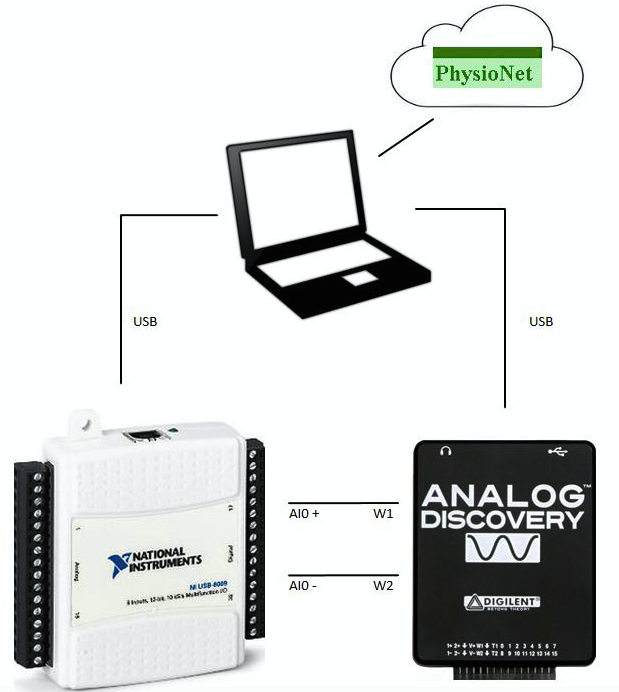
\includegraphics[width=0.5\textwidth]{Figurer/Snip20150427_1}
	\caption{Opstilling af Hardwaren}
\end{figure}

I projektet analyseres virtuelle patienters EKG-signaler. Disse EKG-signaler kommer fra PhysioNet, som er ekstern database, der kan tilgås via internettet\footnote{www.physionet.org}. EKG-signalet, der ønskes analyseres hentes ned som en CSV-fil. Filen's information bliver omdannet til et analog signal, som simuleres af Analog-discovery. Det analoge signal bliver konverters til et digtital signal af DAQ'en. Det er det digitale signal systemet kan afbillede og analysere.
\\ \\
Softwaren for systemet er kernen i dette projekt. Der blev udleveret et program, der anses som en blackbox. Dette program skabes der reference til, således at systemet kan fungere optimalt. Softwaren kan illustrerer og analysere EKG-signaler med henblik på atrieflimren. Systemet kan desuden lagre information om signalerne i en private- og offentlig database.           

